
\documentclass[a4paper, 12pt]{article}
%\usepackage{mathtext}
\usepackage{cmap}
\usepackage[english, russian]{babel}
\usepackage[T2A]{fontenc}
\usepackage[utf8]{inputenc}
\usepackage[left=2cm, right=1.5cm, top=2cm, bottom=2cm]{geometry}
\usepackage{amsmath}
\usepackage{amssymb}
\usepackage{etoolbox}
\usepackage{amsthm}
\usepackage{amsfonts}
\usepackage{mathtools}
%\usepackage{indentfirst}
\usepackage{soulutf8}
\usepackage{graphicx}


\usepackage{tikz,amstext}
\newlength{\tempheight}
\newcommand{\Let}[0]{%
\mathbin{\text{\settoheight{\tempheight}{\mathstrut}\raisebox{0.5\pgflinewidth}{%
\tikz[baseline,line cap=round,line join=round] \draw (0,0) --++ (0.4em,0) --++ (0,1.5ex) --++ (-0.4em,0);%
}}}}

\newcommand{\R}{\mathbb R}
\newcommand{\Q}{\mathbb Q}
\newcommand{\Z}{\mathbb Z}
\newcommand{\N}{\mathbb N}
%\newcommand{\C}{\mathbb C}
\renewcommand{\phi}{\varphi}
\renewcommand{\epsilon}{\varepsilon}
\newcommand{\aug}{\fboxsep=-\fboxrule\!\!\!\fbox{\strut}\!\!\!}
\newcommand\tab[1][.5cm]{\hspace*{#1}}
\newcommand\undermat[2]{\makebox[0pt][l]{$\smash{\underbrace
{\phantom{\begin{matrix}#2\end{matrix}}}_{\text{$#1$}}}$}#2}
\newcommand\overmat[2]{\makebox[0pt][l]{$\smash{\overbrace
{\phantom{\begin{matrix}#2\end{matrix}}}^{\text{$#1$}}}$}#2}

\newcounter{lemcount}
\theoremstyle{definition}
\newtheorem*{definition}{Определение}
\newtheorem*{theorem}{Теорема}%[section]cle
\newtheorem*{consequense}{Следствие}%[theorem]
\newtheorem*{lemma}{Лемма}
\newtheorem*{subtheorem}{Утверждение}
\newtheorem*{remark}{Замечание}
\newtheorem*{example}{Примеры}
\newtheorem*{example1}{Пример}
\newtheorem*{lalala}{Упражнение}
\newtheorem*{algorithm}{Алгоритм}
\newtheorem*{properties}{Свойства}
\newtheorem{lemmanum}[lemcount]{Лемма}

\usepackage[russian]{babel}
\addto\captionsenglish{% Replace "english" with the language you use
  \renewcommand{\contentsname}%
    {Содержание}%
}

\usepackage{titlesec}
\titleformat{\section}{\LARGE \bfseries}{\thesection}{1em}{}
\titleformat{\subsection}{\Large\bfseries}{\thesubsection}{1em}{}
\titleformat{\subsubsection}{\large\bfseries}{\thesubsubsection}{1em}{}

\usepackage{hyperref}
\usepackage{xcolor}
% Цвета для гиперссылок
\definecolor{linkcolor}{HTML}{225ae2} % цвет ссылок
\definecolor{urlcolor}{HTML}{225ae2} % цвет гиперссылок
\hypersetup{
    pdfstartview=FitH, 
    linkcolor=linkcolor,
    urlcolor=urlcolor,
    colorlinks=true
}

\begin{document}
  \begin{titlepage}
    \newpage
    
    \begin{center}
    
\includegraphics[width=4cm]{images.png}
    \end{center}
    
    \vspace{4em}
    
    \begin{center}
    \Large Механико-математический факультет  
    \end{center}
    
    \vspace{2em}
    
    \begin{center}
    \large{\textsc{\textbf{Алгебра, 1 семестр, 2 поток}}}
    \end{center}
    
    \vspace{6em}
    

    
    \newbox{\lbox}
    \savebox{\lbox}{\hbox{Молчанов Вячеслав Вадимович}}
    \newlength{\maxl}
    \setlength{\maxl}{\wd\lbox}
    \hfill\parbox{11cm}
    {
    \hspace*{5cm}\hspace*{-5cm}Преподаватель:\hfill\hbox to\maxl{Куликова Ольга Викторовна\\} \\

    \hspace*{5cm}\hspace*{-5cm}Студент:\hfill\hbox to\maxl{Молчанов Вячеслав\\}\\

    \hspace*{5cm}\hspace*{-5cm}Группа:\hfill\hbox to\maxl{108}
    }
    
    \vspace{\fill}
    
    \begin{center}
    Москва \\2024 
    \end{center}
  \end{titlepage}
  \tableofcontents
  \fontsize{14pt}{20pt}\selectfont
  \newpage
  \fontsize{14pt}{20pt}\selectfont
  \section{Система линейных уравнений}
  \subsection{Матрица. Основные понятия}
  \begin{definition}
    Матрица $A$ размера $m\times n$ это прямоугольная таблица с $m$ строками и $n$ столбцами
    $$ A= \begin{pmatrix}
      a_{11} && a_{12} && \dots && a_{1n}\\
      a_{21} && a_{22} && \dots && a_{2n}\\
      \vdots && \null && \null && \vdots\\
      a_{m1} && a_{m2} && \dots && a_{mn}
    \end{pmatrix}$$ \\
    $a_{ij}$ - элемент матрицы и индексы:

    \begin{itemize}
      \item $i$ - номер строками
      \item $j$ - номер столбца
    \end{itemize}
    
    $M_{m\times n}(\R)$ - Множество всех матриц размера $m\times n$ с элементами из $\R$
    \end{definition}
    Матрица $m\times 1$ называется столбцом:
    $$ A= 
    \begin{pmatrix}
      a_{11} \\
      a_{21} \\
      \vdots \\
      a_{m1} 
    \end{pmatrix} $$
    Если $A=(a_{ij})$ - крадратная, $a_{ij} = 0\ \forall i \neq j$, то $A$ называется диальнольной.
    $$ A =
    \begin{pmatrix}
      a_{11} && \null && \null && 0 \\
      \null && a_{22} && \null && \null \\
      \null && \null && \ddots && \null \\
      0 && \null && \null && a_{nn} 
    \end{pmatrix} $$

    Если $A$ - диальнольная и $a_{ij}$ = 1, то $A$ называется единичной.
    $$ A =
    \begin{pmatrix}
      1 && \null && \null && 0 \\
      \null && 1 && \null && \null \\
      \null && \null && \ddots && \null \\
      0 && \null && \null && 1 
    \end{pmatrix} $$

    \newpage
    %%%%%%%%
    Если $A$ - квадратная, то
    \begin{itemize}
      \item $ A =\begin{pmatrix}
        a_{11} && \null && \null \\
        \null && \ddots && \null \\
        \null && \null && a_{nn} 
      \end{pmatrix} $ главная диагональ
      \item $ A =
      \begin{pmatrix}
        \null && \null && a_{n1} \\
        \null && \dots && \null \\
        a_{n1}  && \null && \null
      \end{pmatrix} $ побочная диагональ
    \end{itemize}
    
    \begin{definition}
      Если $A$ - размера $m\times n$, $a_{ij} = 0\ \forall i,j$, то $A$ называется нулевой.
    \end{definition}

    \subsection{Система линейных (алгебраческих) уравнений}
    $(*)
    \begin{cases}
      a_{11}x_1 + ... + a_{1n}x_n = b_1 \\ 
      a_{21}x_2 + ... + a_{2n}x_n = b_2 \\
      \vdots \\
      a_{n1}x_1 + ... + a_{nn}x_n = b_n
    \end{cases}$ $\\$$\\$
    где $a_{ij}, b \in \R, x_1,... ,x_n$ - неизвестные.
    $$A = \begin{pmatrix}
      a_{11} && \dots && a_{1n} \\
      \vdots && \null && \vdots \\
      a_{n1} && \dots && a_{nn} 
    \end{pmatrix} \hspace{30pt} B = \begin{pmatrix}
      a_{11} \\
      \vdots \\
      b_{n}
    \end{pmatrix}$$
    $A$ - матрица коэфициентов, $a_{ij}$ называется коэфициентом СЛУ.\\
    $B$ - столбец свобоных членов, $b_{j}$ - свободный член.
    \begin{definition}
      Расширенная матрица $\underset{m\times (n+1)}{(A|B)}$. Набор чисел $x_1^0,...,x_n^0 \in \R$ называется решением системы $(*)$, если подстановка этих чисел вместо неизвестных в $(*)$ дает тождество в каждом уравнении. $(x_i^0\longleftrightarrow x)$ 
    \end{definition}
    Решить систему - это найти все решения системы. Любое конткретное решение называется частным.
    \begin{definition}
      Если СЛУ имеет решение, то она называется совместной, иначе несовместной. 
    \end{definition}  
    \begin{definition}
      Совместная система, имеющая одно решение, называется определенной, иначе неопределенной (более одного решения).
    \end{definition}  

    \newpage
    %%%%%%%%
    \subsection{Элементарные преобразования над СЛУ}
    \begin{enumerate}
      \item Прибавить к одному уравнению другое уравнение, умноженное на число $\lambda \in \R$
      \item Поменять местами два уравнения
      \item Умножить уравнение на ненулевое число $\mu \in \R$
    \end{enumerate}
    \begin{subtheorem}
      Эти преобразования обратимы.
    \end{subtheorem}
    \begin{definition}
      Две системы линеных уравнений называются эквивалентными, если их множества решений совпадают.
    \end{definition}
    \begin{subtheorem}
      Если одна СЛУ получена из другой СЛУ с помощью конечного числа элементарных преобразований, то эти системы эквивалентны.
    \end{subtheorem}
    \begin{proof}
      $ \\ \Longrightarrow$ (Не Куликова) 
      $AX = B$ - сходная система, $\tilde{A} X = \tilde{B}$ преобразованная система. \\
      Пусть ${z_1,...,z_n}$ некотороое решение $AX = B$. Будем рассматривать $\tilde{A} X = \tilde{B}$, в ней ЭП $II$ типа умножают строку на $\mu$, имеем:
      $$a_{i1}x_1 +...+ a_{in}x_n = b_{i} \text{ в } AX = B$$
      $$\mu a_{i1}x_1 +...+\mu a_{in}x_n = \mu b_i \text{ в } \tilde{A} X = \tilde{B}$$ 
      Выносим $\mu$ из второго уравнения:
      $$\mu (a_{i1}x_1 +...+ a_{in}x_n) = \mu b_i$$
      Получаем, что ${z_1,...,z_n}$ решение для $\tilde{A} X = \tilde{B}$. Для $III$ типа ЭП очевидно. Теперь рассмотрим $I$ тип, будем к i-ой строчке прибавлять j-ую к коэфициентом $\lambda$, получаем:
      \begin{multline*}
      (a_{i1}+\lambda a_{j1})x_1 +...+(a_{in}+\lambda a_{jn})x_n = \\ = a_{i1}x_1+\lambda a_{j1}x_1 +...+a_{in}x_n+\lambda a_{jn}x_n = \tab[3cm] \\ = a_{i1}x_1 + ... + a_{in}x_n + \lambda (a_{j1}x_1 +...+ a_{jn}x_n) = b_i + \lambda b_j
      \end{multline*}
      Таким образом, любое решение старой СЛУ - это и решение новой, то есть множество
      решений не уменьшилось. (со столбами все тоже самое) \\
      $\Longleftarrow$ В обратную сторону аналогично (для доказательства эквивалентности), используя обратимость элементарных преобразований.
    \end{proof}
    Мораль в том, что мы можем работать с расширенной матрицей $(A|B)$.

    \newpage
    %%%%%%%%
    \subsection{Элементарные преобразования над матрицами}
    \textbf{Элементарные преобразования над строками:} 
    $$A =\begin{pmatrix}
      \overline{a_1} \\
      \overline{a_2} \\
      \vdots \\
      \overline{a_i}
    \end{pmatrix}, \text{ где } \overline{a_i} - \text{строка}$$
    \begin{itemize}
      \item ЭП1: $\overline{a_i} \to \overline{a_i} + \lambda \overline{a_i}$
      \item ЭП2: $\overline{a_i} \longleftrightarrow   \overline{a_j}$
      \item ЭП3: $\overline{a_i} \to \mu \overline{a_i},\ \mu \neq 0$
  \end{itemize}
  \begin{definition}
    Лидер строки (ведущий элемент) - это 1-й ненулевой элемент слева. \\
    \textbf{Пример:} $(0, 0, \underbrace{3}_{\text{лидер}}, 4, 5, 0, 0, 7)$
  \end{definition}
  \begin{definition}
    Матрица $A$ размера $m\times n$ называется ступенчатой, если 
    \begin{enumerate}
      \item Номера лидеров ненулевых строк строго возрастают с увеличением номера строки.
      \item Все нулевые строки стоят внизу (в конце).
    \end{enumerate}
  \end{definition}
  \begin{theorem}
    Любую матрица $A$ размера $m\times n$ за конечное число элементарных преобразований над строками можно привести к ступенчатому виду.
  \end{theorem}
  \begin{proof} Индукция по $n$: \\
    Если $A$ - нулевая, то $A$ - ступенчатого вида. Если $A \neq 0$ : найдем первый ненулевой столбец (начиная слева). Пусть $j$ - номер первого ненулевого столбца. Пусть $a_{ij} \neq 0$: 
    $$A =\begin{pmatrix}
      0 && 0 && \null && \null  \\
      \vdots && \vdots && \null  \\й
      \null && \null && a_{ij} && \null \\
      \vdots && \vdots && \null  \\
      0 && 0 && \null && \null  \\
    \end{pmatrix}$$ 

    \newpage
    %%%%%%%%
    Меняем 1-ю и $i$-ю строку местами и получаем, что $a_{ij}$ стал лидером первой строки. Считаем, что сразу $a_{1j} \neq 0$:
    $$A = \begin{pmatrix}
      0 && 0 && a_{ij} && * \\
      \vdots && \vdots && * && *  \\
      \null && \null && \vdots && \null \\
      \vdots && \vdots && \vdots && \null  \\
      0 && 0 && \vdots && \null  \\  
    \end{pmatrix} $$ \\
    Вычитаем из кажкой $k$-й строки, начиная со 2-ой, 1-ю строку, умноженную на число $\frac{a_{kj}}{a_{1j}}$. Получает вид: 
    $$\tilde{A} =\begin{pmatrix}
      0 && 0 && \vline && * && \null \\
      \vdots && \vdots && \vline && * && * \\
      \null && \null && \vline && \vdots && \null \\
      \vdots && \vdots && \vline && \vdots && \null  \\
      0 && 0 && \vline && \vdots && \null  \\
    \end{pmatrix}$$ \\
    К правой части матрицы применяем индукцию и проводим матрицу к ступенчатому виду.
  \end{proof}
  \begin{remark}
    Этот метод называется  методом Гауса.
  \end{remark}

  \subsection{Решение СЛУ методом Гауса}
  $\begin{cases}
    a_{11}x_1 + ... + a_{1n}x_n = b_1 \\ 
    a_{21}x_2 + ... + a_{2n}x_n = b_2 \\
    \vdots \\
    a_{m1}x_1 + ... + a_{mn}x_n = b_m
  \end{cases}$ \\$\\$
  Элементарные преобразования над $AX=B$ $\Longleftrightarrow$ элементарные преобразования над $(A|B)$. 

  СЛУ $AX=B$ ступенчатая $\Longrightarrow $ $(A|B)$ имеет ступенчатый вид.

  \newpage
  %%%%%%%%
  \begin{subtheorem}
    Решение СЛУ ступенчаного вида.
  \end{subtheorem}  
  Пусть $AX=B$ - ступенчатая
  $$(A|B)=\begin{pmatrix}
    a_{11} & \null & \null & \null & \vline & b_1 \\
    \null & a_{22} & \null & \null & \vline & \vdots \\
    \null & \null & \ddots & \null & \vline & \vdots \\
    \null & \null & \null & a_{sn} & \vline & b_s \\
    \null & \null & \null & \vdots & \vline & \vdots \\
    0 & \cdots & \cdots & 0 & \vline & b_{\widetilde{s}}
  \end{pmatrix}$$ \\
  $\widetilde{s}$ - ненулевые строки расширенной матрицы \\
  s - число ненулевых строк 

  $\widetilde{s}=\left[
    \begin{gathered}
      s \\
      s+1
    \end{gathered}
  \right.$


  \begin{itemize}
    \item[1 случай:]
    $\widetilde{s} \neq s \ (\widetilde{s}=s+1)$ \\ 
    Рассмотрим последнюю ненулевую строку:
    $$\begin{pmatrix}
      a_{11} & \null & \null & \null & \vline & b_1 \\
      \null & a_{22} & \null & \null & \vline & \vdots \\
      \null & \null & \ddots & \null & \vline & \vdots \\
      \null & \null & \null & a_{sn} & \vline & b_s \\
      0 & \cdots & \cdots & 0 & \vline & b_{s+1}
    \end{pmatrix}$$ \\
    $0x_1+...+0x_n=b_{s+1}$ 
    $\Longrightarrow$ решение у этого уравнения нет 
    $\Longrightarrow$ СЛУ не имеет решения, т.е. несовместнаю. \\
    Далее $\widetilde{s}=s$\\
    Заметим, что $\widetilde{s}=s\leq n$ (n-количество столбов)
    \item[2 случай:] $\widetilde{s}=s=n$  
    $$\left\{ \begin{aligned}
      a_{11} x_1 + a_{12} x_2+ \dots + a_{1n} x_n = b_1 \\
      a_{22} x_2 + \dots + a_{1n} x_n = b_2 \\ 
      \ddots \ \ \ \ \ \ \ \ \ \ \ \ \ \ \ \ \vdots \ \\
      a_{nn} x_n = b_n
    \end{aligned}
    \right.$$

    Такая СЛУ называются строго треугольной

    Из n-го уравнения однозначно находится $x_n = \frac{b_n}{a_{nn}}$
    Подставляем во все оставшиеся уравнения $x_n = \frac{b_n}{a_{nn}}$ $\Longrightarrow$ исключаем $x_n$. Получаем строго треугольную систему с меньшим количество неизвестных.  \\
    Далее из (n-1)-го уравнения  находим $x_{n-1}$ и т.д. $\Longrightarrow$ СЛУ имеет единственное решение т.е. является определенной.

    \item[3 случай:] $\widetilde{s}<n$ 
  $$\begin{pmatrix}
    0 & \null & 0 & |\underline{a_{1k_1}} & \ast & \cdots & \cdots & \ast & \vline & \ast  \\
    0 & \null & 0 & 0 & |\underline{a_{2k_2}} & \ast & \cdots & \ast & \vline & \ast \\
    \null & \null & \null & \null & \null & \ddots & \null & \null & \vline & \vdots
  \end{pmatrix}$$ 

  $a_{1k_{1}},...,a_{sk_{s}}$  - лидеры; \\
  $x_{k_{1}},...,x_{k_{s}}$ - главные неизвестные (неизвестные соответствуют лидерам) \\
  Оставшиеся неизвестные назовем свободными. \\
  Перекинем в правую часть СЛУ слагаемые, соответствующие свободным неизвестным 
  $\Longrightarrow$ получаем относительно главных неизвестных строго треугольную СЛУ. \\
  Как в случае 2 однозначно выражается главные неизвестные через свободные
  $\Longrightarrow$ с точностью до нумерации получаем:
  $$\begin{cases}
    x_1 = c_{1,s+1}x_{s+1} + \dots + c_{1n}x_n+d_1 \\
    \vdots \\
    x_s = c_{s,s+1}x_{s+1} + \dots + c_{sn}x_n+d_s
  \end{cases}$$   
  
  Это выражение называется общим решением системы. Подставляя вместо свободных неизвестных конкретное число из $\R$, получаем значение для главных. \\
  $\Longrightarrow$ получаем все решения СЛУ\\
  Если СЛУ имеет > 1 решения - такая СЛУ называется неопределенной. 
  \end{itemize}
  $$\begin{matrix}
    \null &&& \null && \ \ \text{\ \ \ \ СЛУ} \\
    \null && \null && \swarrow && \searrow \\
    &&& \widetilde{s} \neq s && \null &&\widetilde{s} = s\\
    \null &&& \text{несовместна} && \null && \text{совместна} \\
    \null && \null && \null && \swarrow \null && \searrow \\
    \null && \null && \null && \widetilde{s} = s = n \null && \widetilde{s} = s \leq n \\
    \null && \null && \null && \text{определенна} \null && \text{неопределенна}
  \end{matrix}$$
  \begin{algorithm}
    $AX=B \longmapsto (A|B) \thicksim (A_{c}|B_{c})\longmapsto A_cX=B_c$
  \end{algorithm}

  \newpage
  %%%%%%%%
  \begin{definition} 
    Матрица $A$ имеет улучшенный ступенчатый вид, если выполнены следующие условия:
    \begin{enumerate}
      \item $A$ - ступенчатого вида
      \item Все лидеры равны 1
      \item В каждом столбце, где есть лидер $\neq 0$ , все элементы равны 0 
    \end{enumerate}
  \end{definition}  

  \begin{subtheorem}
    Любую матрицу $A$  можно привести к улучшенному ступенчатому виду с помощью элементарных преобразований.
  \end{subtheorem} 
  \begin{proof}
    Т.к. любую матрицу можно привести к ступенчатому виду $\Longrightarrow$ будем считать, что $A$ - ступенчатая. \\
    Рассмотрим последний лидер $a_{sk_s}$. Если $a_{sk_s} \neq 1$, то s-ю строку делим на $a_{sk_s}$ и получаем, что $\widetilde{a_{sk_s}}=1$. \\ Далее из всех строк вычитаем первую, умноженную на $a_{ik_s} \Longrightarrow \widetilde{a_{ik_s}}  =0$ и т.д. 
  \end{proof} 

  \begin{definition}
    СЛУ $AX=B$ называется однородной, если $B=0$, т.е. все свободные члены нулевые.  
  \end{definition} 
  \begin{subtheorem}
    Однородная система всегда совместна.
  \end{subtheorem} 
  \begin{proof}
    $AX=0$ всегда имеет решение $x_1=0,...,x_n=0$ (тривиальное решение)
  \end{proof} 
  \begin{consequense}
    Однородная СЛУ, в которой число уравнений $<$ числа неизвестных, имеет нетривиальное решение.  
  \end{consequense} 
  \begin{proof}
    (в обозначениях из метода Гаусса)\\
    Т.к. система совместна (т.к. $B=0$), то $s=\widetilde{s}$ \\
    С другой стороны $s=\overline{s} \leq$ число исходных уравнений $<$ n $\Longrightarrow s=\widetilde{s} < n \Longrightarrow$ СЛУ неопределенна $\Longrightarrow \exists$ более одного решения $\Longrightarrow \exists$ нетривиальное решение.     
  \end{proof} 

  \newpage
  %%%%%%%%
  \section{Векторные пространства}
  \subsection{Аксиомы элементов векторного пространства}
  Мы рассматриваем векторные пространства над полем $\R$.
  \begin{definition}
    Векторным пространством над $\R$ называют множество элементов $V$, на котором введены операции сложения и умножения на числа из $\R$:
    \begin{enumerate}
      \item $ \forall x,y \in V \Longrightarrow x+y=z \in V$
      \item $\forall \lambda \in \R, \forall x \in V \Longrightarrow \lambda x = w \in V$ 
    \end{enumerate}
    Удовлетворяет следующими свойствами:
    \begin{enumerate}
      \item x+y = y+x (коммутативность)
      \item (x+y)+z = x+(y+z) (ассоциативность)
      \item $\exists \tab[0.1cm] 0 \in V: \forall x \in V: x+0 = 0+x = x$ (нейтральный элемент относильно сложения)
      \item $\forall x \in V: \exists \tab[0.1cm] x^{\prime}: x + x^{\prime} = 0$ (противоположный элемент)
      \item $\forall \lambda \in \R, \forall x,y \in V: \lambda (x+y) = \lambda x + \lambda y$ (дистрибутивность умножения отностильно сложения)
      \item $\forall \lambda, \mu \in \R, \forall x \in V: (\lambda+\mu)x = \lambda x + \mu x $ (дистрибутивность сложения отностильно умножения)
      \item $\forall \lambda, \mu \in \R, \forall x \in V: \lambda(\mu x) = (\lambda \mu) x $ (ассоциативность умножения)
      \item $\forall x \in V: 1 \cdot x = x$ (нейтральный элемент относильно умножения)
    \end{enumerate}
  \end{definition} 

  \begin{definition}
    Любой элемент векторного пространства называется вектором.
  \end{definition} 

  \textbf{Примеры векторных пространств:} 
    \begin{enumerate} 
      \item $V^2$ - Геометрические векторы на плоскости.
      \item $V^3$ - Геометрические векторы в пространстве.
      \item $\R^n$ = $\{ {(a_1,...,a_n) | a_i \in \R} \}$ - арифметические векторы.
    \end{enumerate}
    \tab[0.8cm]"$+$": $(a_1,...,a_n)$ + $(b_1,...,b_n)$ = $(a_1+b_1,...,a_n+b_n)$ \\
    \tab[0.8cm]"$\times$": $(a_1,...,a_n) \times \lambda$ = $(a_1\lambda,...,a_n\lambda)$ 
  \begin{lalala}
    Проверьте, что $\R^n$ (арифметическое пространство строк) с этими операциями является векторным пространством. 
  \end{lalala}  
  \subsection{Следствия}
  \begin{enumerate}
    \item нулевой вектор единственный
    \begin{proof}
      Пусть существует два $\overline{0}_1,\overline{0}_2 \in V$, тогда: $$\overline{0}_2 = \overline{0}_1 + \overline{0}_2 = \overline{0}_2 + \overline{0}_1 = \overline{0}_1$$   
    \end{proof} 
    \item $\forall x \in V$ противоположный вектор единственный
    \begin{proof}
      Пусть существует два $x_1,x_2$ - различные противоположные к вектору $x$, тогда:
      $$\overline{0} + x_2 = (x_1 + x) + x_2 = x_1 + (x + x_2) = x_1 + \overline{0}$$    
    \end{proof} 
    \item $\forall \lambda \in \R: \lambda \cdot \overline{0} = \overline{0}$ 
      \begin{proof}
      $$\lambda \cdot \overline{0} = \lambda \cdot (\overline{0}+\overline{0}) = \lambda \cdot \overline{0} + \lambda \cdot \overline{0}$$ Прибавим к обе им частям уравнения $\lambda \cdot \overline{0} = \lambda \cdot \overline{0} + \lambda \cdot \overline{0}$  противоположный к $\lambda \cdot \overline{0}$, тогда: $$\lambda \cdot \overline{0} + (-\lambda \cdot \overline{0})= \lambda \cdot \overline{0} + \lambda \cdot \overline{0} + (-\lambda \cdot \overline{0})$$ $$\overline{0} = \lambda \cdot \overline{0}$$ 
      \end{proof} 
    \item $\lambda \cdot (-x) = -\lambda \cdot x$
    \item $\lambda \cdot (x-y) = \lambda x - \lambda y$ 
    \item $\lambda \cdot \overline{0} = \overline{0}$
    \item $(-1) \cdot x = -x$
    \item $(\lambda - \mu)\cdot x = \lambda x - \mu x$  
  \end{enumerate}
  \subsection{Векторные подпространства}
  \begin{definition}
    Подмножество $U\subseteq V$ над векторным подпространством, если:
    \begin{enumerate}
      \item $ x, y \in U \Longrightarrow  x + y \in U$ 
      \item $\forall \lambda \in \R, \forall x \in U \Longrightarrow \lambda \cdot x \in U$ 
      \item $U \neq \varnothing$ 
    \end{enumerate}
  \end{definition} 
  \begin{remark}
    3 условие заменить на условие: $0 \in  U$
    \begin{itemize}
      \item [$\underline{\Longleftarrow}$] очевидно.
      \item [$\underline{\Longrightarrow}$] если $U \neq \varnothing$, то $\exists \tab[0.1cm] x \in U \Longrightarrow$ по $2.: (-1) \cdot x \in U \Longrightarrow -x \in U  \Longrightarrow \\ x + (-x) \in U \Longrightarrow 0 \in U$ 
    \end{itemize}
  \end{remark} 
  \begin{subtheorem}
    Любой вектор подпространства векторного пространства $V$ сам является векторным пространством относительно операций векторного пространства 
  \end{subtheorem} 
  \begin{proof}
    Надо проверить определение. 1 и 2 свойство из операций векторного пространства означают, что в $U$ заданы операции сложения и умножения на вещественное число. Проверка аксиом векторного пространства: 1,2,5,6,7,8 выполнены для всех векторов из $V$, а значит и для всех векторов из $U$. \\ 3,4 доказательство как в замечании. 
    $$\forall x \in U, \ \exists \tab[0.1cm](-x) = (-1) \cdot x \in U, \ \overline{0} \in U, \text{ т.к. } U \neq \varnothing $$   
  \end{proof} 
  \begin{example} \end{example}
    \begin{enumerate} 
      \item $V^3, U$ - множество всех векторов из $V^3$, параллельные фиксированной плоскости.
      \item $\R^n, U=\{(a_1,..., a_n) | a_{2i} = 0\}$ - векторное подпространство \\ $\widetilde{U} = \{(a_1,..., a_n) | a_{2i} = 1\}$ - не векторное подпространство, т.к. множество не замкнуто относительно сложения и умножения.
      \item В любом векторном простанстве $V$ есть такие подпространства, состоящие только из нулевого вектора. (тривиальное или несобственное подпространство) (Остальное называется собственными)
    \end{enumerate}
  
  \newpage
  %%%%%%%%
  \subsection{Линейная зависимость системы векторов}
  $V$ - векторное пространство над полем $\R$
  \begin{definition}
    Линейной комбинацией векторов $v_1,...,v_n \in V$ с коэфициентами $\lambda_1,...,\lambda_n \in \R$ называется выражение вида: 
    $$\lambda_1 x_1 + \cdots + \lambda_n x_n$$ 
    Говорят, что вектора $w \in V$ линейно выражается через $(v_1,...,v_n)$, \\ если $\exists\tab[0.1cm]\lambda_1,...,\lambda_n \in \R: w = \lambda_1 x_1 + \cdots + \lambda_n x_n$   
  \end{definition}   
  \begin{definition}
    Линейной комбинацией $\lambda_1 x_1 + \cdots + \lambda_n x_n$ назавается тривиальной, если $\lambda_1 = 0,...,\lambda_n = 0$. Иначе нетривиальной.
  \end{definition}
  \begin{definition}
    Система векторов $v_1,...,v_n$ называется линейно зависимой (ЛЗ), если $\exists$ нетривиальная линейная комбинация равная 0, (т.е. $\exists \tab[0.1cm]\lambda_1,...,\lambda_n \in \R$ не все равные 0) такая что $\lambda_1 x_1 + \cdots + \lambda_n x_n = 0$. Иначе система называется линейно независимой (ЛНЗ), т.е. из любого такого равенства $\lambda_1 x_1 + \cdots + \lambda_n x_n = 0 \\ \Longrightarrow (\lambda_1,...,\lambda_n) = 0$.
  \end{definition}
  \begin{example}
    $V^2, v_1 = i + j, v_2 = 2i, v_3 = 3i$ -линейно зависимая система, т.к. $$1 \cdot (i + j) + (- \frac{1}{2}) \cdot (-\frac{1}{3}) \cdot (3i) = 0$$ $$1 \cdot v_1 + (-\frac{1}{2}) \cdot v_2 + (-\frac{1}{3}) \cdot v_3 = 0$$  
  \end{example}  
  \begin{properties} \end{properties} 
    \begin{enumerate}
      \item Система из одного вектора $V_1$ ЛЗ $\Longleftrightarrow V_1 = 0$  
      \item Система из 2-х векторов $v_1 \text{и} v_2$ ЛЗ $\Longleftrightarrow$ противоположные, т.е. $v_1 = \lambda v_2 \\ v_2 = \mu v_1$. 
    \end{enumerate}
  \begin{example1}
    $\R^n$ \\
    Система $\underbrace{(1,0,0,...,0)}_{e_1} , \underbrace{(0,1,0,...,0)}_{e_2},...,\underbrace{(0,0,0,...,1)}_{e_n}$ линейно независимая \\
    $\lambda_1 e_1 + \cdots + \lambda_n e_n = (0,...,0) \Longleftrightarrow (\lambda_1,...,\lambda_n) = 0 \Longleftrightarrow $ ЛНЗ 
  \end{example1}
  \begin{lemmanum}
    (Критерий линейной зависимости)
    Система векторов $v_1,...,v_n \in V, \\ n>1$ - линейно зависимы $\Longleftrightarrow $ хотя бы один вектор линейно выражается через оставшиеся.  
  \end{lemmanum} 

  \newpage
  %%%%%%%%
  \begin{proof} $\tab$  
    \begin{itemize}
      \item[$\underline{\Longrightarrow}$]
      По определению ЛЗ $\exists \tab[0.1cm] \lambda_1,...,\lambda_n \in \R$ не все нулевые: $\lambda_1 v_1 + \cdots + \lambda_n v_n = 0$. Без ограничения общности можем считать, что $\lambda_1 \neq 0$, тогда $v_1 = \frac{1}{\lambda_1}(-\lambda_2 v_2 - \cdots - \lambda_n v_n)$
      \item[$\underline{\Longleftarrow }$] Пусть один из этих векторов выражается через оставшиеся. Без ограничения общности можем считать, что $v_1$ выражается через оставшиеся \\ $v_1 = \mu_2 v_2 + \cdots + \mu_n v_n$ \\ $1 \cdot v_1 -\mu v_2 - \cdots - \mu_n v_n = 0$ - нетривиальная линейнвая комбинация, \\ т.к. $\mu_1 (\text{коэф. перед }v_1) \neq 0 \Longrightarrow {v_1,...,v_n}$ - линейно зависима.
    \end{itemize}  
  \end{proof} 
  \begin{remark}
    В лемме 1 нельзя <<хотя бы один>> заменить на <<любой>>! \\
    Пусть $v_1 \neq 0, v_2 = 0$ и $v_1, v_2$ - ЛЗ, т.к. $0 \cdot v_1 + 1 \cdot v_2 = 0$
  \end{remark} 
  \begin{lemmanum} \label{lem2}
    Пусть $v_1,...,v_n \in V$ - ЛНЗ, тогда $w \in V$ линейно выражается через $v_1,...,v_n \Longleftrightarrow (w,v_1,...,v_n)$ - ЛЗ.   
  \end{lemmanum} 
  \begin{proof} $\tab$  
    \begin{itemize}
      \item[$\underline{\Longrightarrow}$] $\exists \tab[0.1cm] \mu_1,...,\mu_n \in \R: w = \mu_1 v_1 + \cdots +\mu_n v_n \Longrightarrow$ по критерию ЛЗ система $\{w,v_1,...,v_n\}$ - ЛЗ.
      \item[$\underline{\Longleftarrow}$] Пусть система ЛЗ $\Longrightarrow \exists \tab[0.1cm] \lambda_0,...,\lambda_n \in \R$ - не все нули, так что  $\lambda_0 w + \lambda_1 v_1 + \cdots + \lambda_n v_n = 0$, тогда: 
      \begin{enumerate}
        \item $ \lambda_0 = 0$, то $\lambda_1 v_1 + \cdots + \lambda_n v_n = 0$ - нетривиальная линейная комбинация
        \item $\lambda_0 \neq 0 \Longrightarrow w = (-\frac{\lambda_1}{\lambda_0})v_1 + \cdots + (-\frac{\lambda_n}{\lambda_0})v_n$
      \end{enumerate} 
    \end{itemize}
  \end{proof}
  %%
  \begin{lemmanum} \label{lem3}
    Пусть вектор $w$ линейно выражается через $v_1,..,v_k$. Тогда это выражение единственное.   
  \end{lemmanum} 
  \begin{proof} $\tab$ 
    \begin{itemize}
      \item[$\underline{\Longrightarrow}$] Пусть выражается единственно. Допустим, $v_1,..,v_k$ - ЛЗ $\Longrightarrow \exists\{\lambda_1,..,\lambda_k\}$ не все нулевые, т.ч. $\lambda_1v_1 + \cdots + \lambda_kv_k=0$ \\
      Тогда если $w=\mu_1v_1 + \cdots + \mu_kv_k$, то $w + 0 = (\mu_1+\lambda_1)v_1 + \cdots + (\mu_k + \lambda_k)v_k$ другое разложение, противоречие.  
      \item[$\underline{\Longleftarrow}$] Пусть $v_1,..,v_k$ - ЛНЗ. Допустим, что существует два разложения: $$w = \mu_1v_1 + \cdots + \mu_kv_k$$  $$w = \widetilde{\lambda_1}v_1 + \cdots + \widetilde{\mu_k}v_k$$ 
      $\Longrightarrow  \{v_1,..,v_k\}$ - ЛЗ $\Longrightarrow $ противоречие.
    \end{itemize}
  \end{proof}
  \begin{lemmanum} $\tab$
    \begin{enumerate}
      \item Если какая-то подсистема векторов ЛЗ, то вся система ЛЗ.
      \item Если система векторов ЛНЗ, то любая подсистема ЛНЗ.
    \end{enumerate}
  \end{lemmanum}  
  \begin{proof} $\tab$ 
    \begin{enumerate}
      \item Пусть подсистема $v_1,..,v_k$ системы $v_1,..,v_k,...,v_m$ - ЛЗ $\Longrightarrow \exists \lambda_1,...,\lambda_k$ не все равные нулю, т.ч. $\lambda_1v_1 + \cdots _+ \lambda_kv_k=0$ Положим $\lambda_{k+1}=0,...,\lambda_m=0$ 
      Тогда $\lambda_1v_1,..,\lambda_kv_k,...,\lambda_mv_m=0$ - нетривиальная ЛК $\Longrightarrow \{v_1,...,v_k,v_{k+1},...,v_m\}$ - ЛЗ. 
      \item Следует из 1.
    \end{enumerate}
  \end{proof} 
  \begin{lemmanum} (ОЛЛЗ) \\
    Пусть $v_1,...,v_k \in V, w_1,...,w_m \in V$, причем каждый $w_i$ линейно выражается через $v_1,...,v_k$, тогда, если $m>k$, то $\{w_1,...,w_m\}$ - ЛЗ.  
  \end{lemmanum} 
  \begin{proof}
    Пусть 
    $$\begin{cases}
      w_1 = c_{11}v_1+\cdots+c_{1k}v_k \\
      w_2 = c_{21}v_1+\cdots+c_{2k}v_k \\
      \vdots \\
      w_m = c_{m1}v_1+\cdots+c_{mk}v_k
    \end{cases}
    \text{где } c_{ij} \in \R
    $$
    Докажем, что $\exists$ нетривиальная ЛК $w_1,...,w_m=0$ \\
    Для произвольных $\lambda_1,...,\lambda_m$ рассмотрим выражение: 
    \begin{multline*}
      \lambda_1w_1 +\cdots+\lambda_mw_m = \\ = \lambda_1(c_{11}v_1+\cdots+c_{1k}v_k) + \cdots + \lambda_m(c_{m1}v_1+\cdots+c_{mk}v_k) = \\ = (\lambda_1c_{11}+\cdots+\lambda_mc_{m1})v_1+\cdots+(\lambda_1c_{1k}+\cdots+\lambda_mc_{mk})v_k 
    \end{multline*}
    Рассмотрим СЛУ с неизвестными $\lambda_1,...,\lambda_m$ из $k$ уравнений:
    $$\begin{cases}
      c_{11}\lambda_1+\cdots+c_{m1}\lambda_m=0 \\
      \vdots \\
      c_{1k}\lambda_1+\cdots+c_{mk}\lambda_m=0
    \end{cases}$$ 
    Т.к. $m>k$ и это ОСЛУ в которой число уравнений $<$ числа неизвестных, то эта система имеет нетривиальное решение \\
    $\lambda_1,...,\lambda_m \Longrightarrow \lambda_1w_1+\cdots+\lambda_mw_m = 0$ - это нетривиальная ЛК \\ $\Longrightarrow w_1,...,w_m$ - ЛЗ. 
  \end{proof} 
  \subsection{Линейная оболочка множества S}
  $V$ - векторное простанство над $\R$ \\
  $S \subseteq V, S \neq \varnothing $ 
  \begin{subtheorem}
    Множество всех ЛК $\lambda_1s_1+\cdots+\lambda_ks_k,\tab[0.1cm] \lambda_i \in \R,\tab[0.1cm] s_i \in S$ образует векторное подпространство в пространстве $V$. 
  \end{subtheorem}  
  \begin{proof}
    Д/з. 
  \end{proof}
  \begin{definition}
    Такое векторное подпространство называется линейная оболочка множества $S$, обозначается $\langle S \rangle$.
  \end{definition} 
  \begin{example} $\tab$ 
    \begin{enumerate}
      \item $\R^3,\tab[0.1cm] S = \{(1,0,0),(0,1,0)\};$ \tab[0.5cm]
      $\langle S \rangle = \{(\lambda,\mu,0)\tab[0.1cm]|\tab[0.1cm]\lambda,\mu \in \R\}$ 
      \item $V^3,\tab[0.1cm] S =\{i,j,i+j\}$ \\ $\\$  
      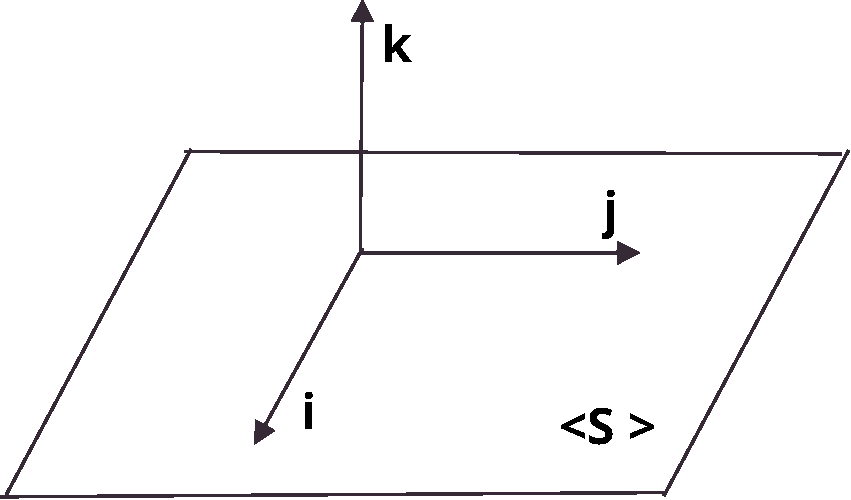
\includegraphics[width=6cm]{.v3.pdf} $\widetilde{s} = \{i+j\}$ 
    \end{enumerate}
  \end{example}
  \begin{definition}
    Если $V=\langle S \rangle$, то $S$ называется порождающим множеством векторного простанства $V$. Говорят векторное пространство $V$ порождается множеством $S$. 
  \end{definition} 
  \begin{definition}
    Если $\exists$ конечное множество $S$, т.ч. $V=\langle S \rangle$, то $V$ называется конечномерным (конечнопорожденным), иначе бесконечномерным.
  \end{definition} 
  \begin{example1}
    $\R^n = \langle (1,0,...,0),...,(0,...,0,1) \rangle$ 
  \end{example1}
\begin{lemma} (Переформулировка ОЛЛЗ)
  Пусть векторное пространство $V$ пораждается $k$ векторами. Тогда любые $m>k$ векторов из $V$ - ЛЗ.
\end{lemma} 
\subsection{Базис}
$V$- конечномерное векторное простанство над $\R$ 
\begin{definition}\tab[-0.1cm]\textbf{1} 
  Система векторов $\{e_1,...,e_n\}\subseteq V$ называется бизисом векторного пространства $V$, если:
  \begin{enumerate}
    \item $\{e_1,...,e_n\}$ - ЛНЗ
    \item $V = \langle e_1,...,e_n \rangle$, т.е. $\forall x \in V, \tab[0.1cm] \exists \tab[0.1cm] x_1,...,x_n \in \R: x = x_1e_1+\cdots + x_ne_n$  
  \end{enumerate}
  Эти числа $x_1,...,x_n$ - называются координатами вектора $x$ в базисе $\{e_1,...,e_n\}$ 
\end{definition} 
\begin{definition}\tab[-0.1cm]\textbf{2} 
  Система векторов $\{e_1,...,e_n\} \subseteq V$ называется базисом векторного простанства $V$, если любой вектор $x \in V$ выражается через $\{e_1,...,e_n\}$ единственным образом.
\end{definition} 
  \begin{subtheorem}
    (\textbf{Опр 1}) $\Longleftrightarrow $ (\textbf{Опр 2})
  \end{subtheorem} 
  \begin{proof}
    По лемме \eqref{lem3}.
  \end{proof}
  \begin{theorem}
    Всякое конечномерное векторное пространство над $\R$ обладает базисом. Более того, из любого конечного порожденного множества можно выбрать базис.
  \end{theorem} 
  \begin{proof}
    Пусть $S$- какое-то порожденное множество векторного пространства $V$. \\
    Если $S$ - ЛНЗ, то $S$ - базис \\
    Если $S$ - ЛЗ, то по критерию о ЛЗ один из векторов $S_1$ множества $S$ линейно выражается через остальные. \\
    Тогда $S_1$ = $S\setminus\{s_1\}$ - конечное пораждащее множество. ч.т.д. \\
    Т.к. $S$ - конечное, это процесс прервется и мы получим ЛНЗ порожденную систему.
  \end{proof} 
  \begin{theorem}
    В любом базисе конечномерного векторного пространства $V$ над $\R$ одно и тоже число векторов.
  \end{theorem} 
  \begin{proof}
    Пусть есть два базиса $\{e_1,...,e_m\}$ и $\{f_1,...,f_m\}$ векторного пространства $V$. 
    Тогда каждый вектор $f_i$ выражается через $e_1,...,e_m$. \\
    По ОЛЛЗ: $\{f_1,...,f_m\}$ - ЛЗ $\Longrightarrow \{f_1,...,f_m\}$ - не базис $\Longrightarrow $ противоречие.  
  \end{proof} 
  \begin{definition}
    Число векторов в базисе конечномерного векторного пространства $V$, называется размерностью векторного простанства и обозначается: $dimV$ 
  \end{definition} 
  \begin{example} $\tab$ 
    \begin{enumerate}
      \item $dimV^2 = 2$
      \item $dim \R^n = n$   
    \end{enumerate}
  \end{example}
  \begin{remark}
    Если $V={0}$, то $dimV = 0$ (базис систоит из $\varnothing$ ) 
  \end{remark} 
   Пусть $V$- векторное пространство над $\R$, $dimV=n,\tab[0.1cm] S\subseteq V$ Любые $m>n$ векторов в $S$ - ЛЗ. (из ОЛЛЗ) \\
   $\Longrightarrow $ в $S \ \exists $ максимальная ЛНЗ подсистема (т.е. ничего нельзя добавить к этой подсистеме без нарушения ЛНЗ) 
  \begin{lemmanum} \label{lem6}
    Пусть $V$ - n-мерное векторное пространство над $\R,\tab[0.1cm] S\subseteq V$. Тогда максимальная ЛНЗ система векторов из $S$ образует базис в лин. оболочке $\langle S \rangle$  
  \end{lemmanum} 
  \begin{proof}
    Пусть $\{s_1,...,s_k\}$ максимальная (по включению) ЛНЗ система в $S$ $\Longrightarrow \forall s \in S \setminus \{s_1,...,s_k\}\Longrightarrow \{s,s_1,...,s_k\} - \text{ЛЗ.} $ \\
    По Лемме \eqref{lem2}. $\Longrightarrow s=\lambda_1s_1+\cdots+\lambda_ks_k$ \\
    Докажем, что $\{s_1,...,s_k\}$ базис в $\langle S \rangle$. 
    \begin{enumerate}
      \item ЛНЗ (очевидно)
      \item $\forall x \in \langle S \rangle\tab[-0.1cm]: x = x_1s_1+\cdots+x_ks_k$ 
    \end{enumerate}
    По определению линейной оболочки $x$ линейно выражается через вектора из $S$ \\
    А каждый вектор из $S$ линейно выражается через $\{s_1,...,s_k\}$ 
  \end{proof}
  \begin{theorem}
    Пусть $V$ конечномерное векторное пространство над $\R$, тогда:
    \begin{enumerate}
      \item Любая максимальная ЛНЗ система векторов из $V$ - базис $V$.
      \item Любую ЛНЗ систему векторов из $V$ можно дополнить до базиса векторного пространства $V$. 
    \end{enumerate}
  \end{theorem}  
  \begin{proof} $\tab$ 
    \begin{enumerate}
      \item По лемме \eqref{lem6}. $S=V$ 
      \item Пусть $S$ - ЛНЗ система векторов из $V$ 
    \end{enumerate}
    Если $V=\langle S \rangle$, тогда $S$- базис. \\
    Если $V \neq \langle S \rangle$ , то $\exists s_1 \in V \setminus \langle S \rangle$ \\
    $\Longrightarrow s_1$ линейно невыражается через $S$ $\Longrightarrow \text{(По лемме \ref{lem2}.) } S_1=S \cup \{s_1\}$ - ЛНЗ. \\
    $\Longrightarrow $ Если $V = \langle S \rangle$, то $S_1$ базис, иначе $\exists S_2 \in V \setminus \langle S_1 \rangle$, и т.д. \\
    Этот процесс прервется на конечном шаге, т.к. пространство $V$- конечное. (Если $dimV \neq n, \text{то} \not\exists$ ЛНЗ системы с числом векторов $> n$) 
  \end{proof} 
  \begin{consequense} 
    Пусть $V$ конечномерное векторное пространство над $\R$ 
    \begin{enumerate}
      \item Любой ненулевой вектор можно дополнить до базиса.
      \item Любые $n$ ЛНЗ вектора в $n$-мерном пространстве $V$ образуют базис.
    \end{enumerate}
  \end{consequense} 
  
  \section{Ранг}
  \begin{definition}
    Рангом системы векторного простанства $S\subseteq V$ называется $dim \langle S \rangle$  
  \end{definition} 
  $A$ - матрица $m \times n$ \\ $\\$
  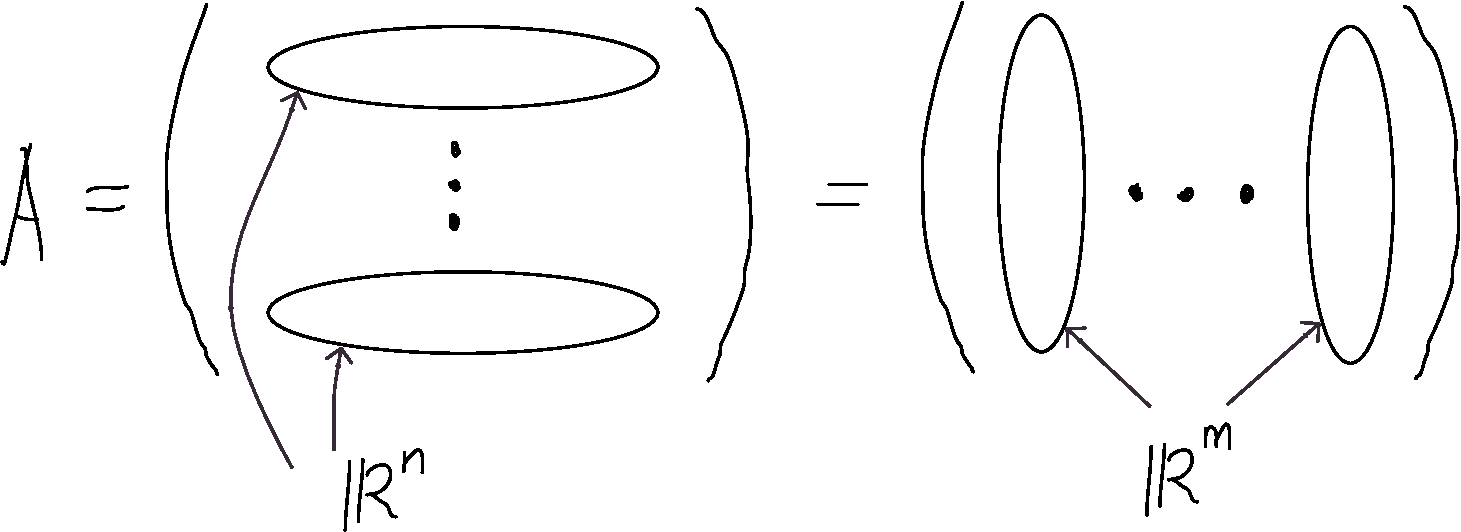
\includegraphics[width=15cm]{.matr.pdf}
  \begin{definition}
    Рангом матрицы $A$ называется ранг системы ее строк, т.е. максимальное число ЛНЗ строк матрицы.
  \end{definition} 


  \section{Мораль в том, что я не успел....}
   
\end{document}


